% ==========================================================
% Póster del proyecto Bioactive (A1 horizontal, 3 columnas).
% Parte de la plantilla del curso (Poster.zip, Canvas): se conservan el encabezado
% institucional, la paleta, la tipografía y el tamaño de fuente; cambian el contenido y,
% como permite la rúbrica, la distribución y los títulos de las secciones.
% Compilación: sh scripts/compilar_articulo.sh poster
% ==========================================================
\documentclass[10pt]{article}

\usepackage{iftex}
\usepackage[a1paper,landscape,margin=1.5cm]{geometry}
\usepackage[spanish,es-noshorthands]{babel}
\usepackage{xcolor}
\usepackage{graphicx}
\usepackage{tikz}
\usetikzlibrary{arrows.meta}
\usepackage[most]{tcolorbox}
\usepackage{enumitem}
\usepackage{booktabs}
\usepackage{colortbl}
\usepackage{microtype}
\usepackage[hidelinks]{hyperref}

\ifTUTeX
  \usepackage{fontspec}
  \IfFontExistsTF{Instrument Serif}%
    {\newfontfamily\serif{Instrument Serif}}%
    {\newfontfamily\serif{TeX Gyre Pagella}}
\else
  \usepackage[utf8]{inputenc}
  \usepackage[T1]{fontenc}
  \usepackage{lmodern}
  \usepackage[scaled=0.95]{helvet}
  \newcommand{\serif}{\fontfamily{bch}\selectfont}
\fi

\pagestyle{empty}
\setlength{\parindent}{0pt}
\setlength{\parskip}{0.4em}

% ---------------------- PALETA (de la plantilla) ------------
\definecolor{olive}{HTML}{9AA542}
\definecolor{olivedark}{HTML}{1B2208}
\definecolor{olivelink}{HTML}{6B7A1F}
\definecolor{olivesoft}{HTML}{E4E8C7}
\definecolor{ink}{HTML}{1A1A10}
\definecolor{muted}{HTML}{6B6B5E}
\definecolor{pagebg}{HTML}{FFFFFF}
\definecolor{alerta}{HTML}{E8672B}       % el naranja de las figuras: lo que no cuadra

\pagecolor{pagebg}
\color{ink}

% ---------------------- DATOS DEL PÓSTER -------------------
\newcommand{\programa}{Maestría en Inteligencia Artificial Aplicada}
\newcommand{\tituloA}{Bioactive}
\newcommand{\tituloB}{Cuánto confiar en una predicción depende de la molécula, no del modelo}
\newcommand{\autores}{Ingrid Pamela Ruiz Puga\quad Artemio Santiago Padilla Robles\quad José Antonio Vázquez Martínez}
\newcommand{\asesor}{Dra. Grettel Barceló Alonso}
\newcommand{\patrocinadora}{Dra. Mariana Martínez Ávila}
\newcommand{\fecha}{Noviembre 2026}

\newcommand{\logoizq}{
\includegraphics[height=5cm]{logo.jpeg}}
\newcommand{\logoder}{
\includegraphics[height=5cm]{logo_der.png}}

% ---------------------- ESTILOS ----------------------------
\newcommand{\seccion}[1]{%
  \begin{tcolorbox}[colback=olive,colframe=olive,arc=0pt,
    boxrule=0pt,left=8pt,top=3pt,bottom=4pt,width=\linewidth]
    {\serif\color{white}\fontsize{30}{36}\selectfont #1}
  \end{tcolorbox}\vspace{-0.3em}}

\newcommand{\circulo}[2]{%
  \tikz\node[circle,fill=olivesoft,minimum size=5.6cm,align=center,text width=4.8cm,text=olivedark]{{\serif\fontsize{40}{44}\selectfont #1}\\[2pt]{\sffamily\bfseries\fontsize{19}{23}\selectfont #2}};}

\newcommand{\cuerpo}{\fontsize{22}{28}\selectfont}
\newcommand{\pie}[1]{{\sffamily\fontsize{18}{22}\selectfont\color{muted}#1}}

\newlength{\hdrh}\setlength{\hdrh}{9cm}
\newlength{\colh}
\setlength{\colh}{\dimexpr\textheight-\hdrh-6cm\relax}

% ======================================================
\begin{document}

% ---------------------- ENCABEZADO ------------------------
\noindent\parbox[t][\hdrh][c]{\linewidth}{%
\begin{minipage}[c]{0.20\linewidth}
  \raggedright\logoizq
\end{minipage}%
\begin{minipage}[c]{0.60\linewidth}
  \centering
  {\serif\fontsize{58}{65}\selectfont\color{olivedark}%
   \tituloA\\\fontsize{40}{46}\selectfont\tituloB\par}
  \vspace{0.5em}
  {\sffamily\bfseries\fontsize{30}{36}\selectfont\color{olivelink}\programa\par}
  \vspace{0.3em}
  {\fontsize{26}{32}\selectfont\color{ink}\autores\par}
  {\fontsize{22}{28}\selectfont\color{muted}Asesora: \asesor\ \textperiodcentered\ Patrocinadora: \patrocinadora\ \textperiodcentered\ \fecha\par}
\end{minipage}%
\begin{minipage}[c]{0.20\linewidth}
  \raggedleft\logoder
\end{minipage}}

\vspace{0.4cm}
{\color{olive}\rule{\linewidth}{2.5pt}}
\vspace{0.6cm}

% ---------------------- COLUMNAS --------------------------
\noindent
\begin{minipage}[t][\colh][s]{0.30\linewidth}\cuerpo\vspace{0pt}
% ===== COLUMNA IZQUIERDA =====

\seccion{El problema}
Probar en el laboratorio cada compuesto natural con potencial neuroprotector es lento y caro. Para decidir cuáles probar primero, dos modelos estiman, a partir de su estructura química, si un compuesto:

\begin{itemize}[leftmargin=1.2em,itemsep=0.4em]
  \item cruza la barrera que protege al cerebro (fase 1);
  \item actúa sobre alguna de 26 proteínas del sistema nervioso, y con qué potencia (fase 2).
\end{itemize}

\vspace{0.2em}
\begin{center}
\begin{tikzpicture}[
  caja/.style={draw=olive,fill=olivesoft,rounded corners=4pt,line width=2pt,align=center,
    font=\sffamily\bfseries\fontsize{19}{23}\selectfont,text=olivedark,minimum height=2.6cm,text width=5.0cm},
  arr/.style={-{Stealth[length=4mm]},line width=3pt,color=olive}]
  \node[caja,fill=white] (a) at (0,0) {Estructura\\del compuesto};
  \node[caja] (b) at (6.6,1.55) {Fase 1: ¿cruza\\la barrera?};
  \node[caja] (c) at (6.6,-1.55) {Fase 2: ¿con qué\\potencia actúa?};
  \node[caja,fill=white] (d) at (13.2,0) {Evidencia para\\priorizar};
  \draw[arr] (a.east) -- (b.west);
  \draw[arr] (a.east) -- (c.west);
  \draw[arr] (b.east) -- (d.west);
  \draw[arr] (c.east) -- (d.west);
\end{tikzpicture}
\end{center}
La salida es evidencia para decidir en qué orden probar, no una decisión automática.

\vfill
\seccion{Datos}
\begin{center}
  \circulo{7,805}{compuestos\\(fase 1)}\hspace{0.6cm}\circulo{202,647}{mediciones\\(fase 2)}
\end{center}
\begin{itemize}[leftmargin=1.2em,itemsep=0.5em]
  \item Fase 1: archivo curado de la patrocinadora (63.5\,\% permeables). Fase 2: ChEMBL, NPASS y CMAUP, con mediciones acotadas (por ejemplo, mayores que 10 µM).
  \item Prueba reservada de 1,499 compuestos que ningún modelo vio; la separación es por familia química, nunca al azar.
\end{itemize}

\vfill
\seccion{Métodos}
\begin{itemize}[leftmargin=1.2em,itemsep=0.5em]
  \item Descriptores de RDKit (propiedades calculadas de cada molécula) y, en la fase 2, huellas de Morgan. Once modelos comparados, de la regresión logística a los ensambles.
  \item En la fase 2, un modelo que aprovecha también las mediciones acotadas, que solo dicen que el valor es mayor o menor que un límite.
\end{itemize}

\end{minipage}\hfill
\begin{minipage}[t][\colh][s]{0.37\linewidth}\cuerpo\vspace{0pt}
% ===== COLUMNA CENTRAL =====

\seccion{Lo que encontramos}
\begin{minipage}[t]{0.485\linewidth}\centering
  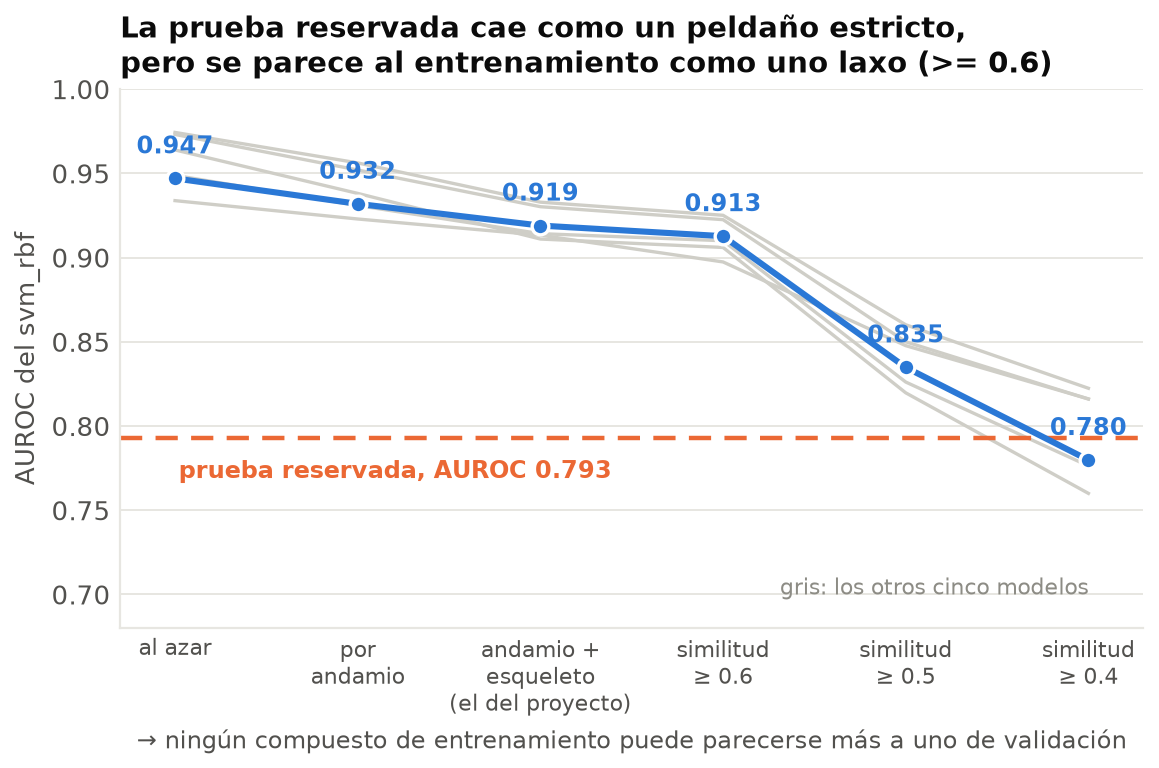
\includegraphics[width=\linewidth,height=9.8cm,keepaspectratio]{f1_escalera.png}\\[2pt]
  \raggedright\pie{Figura 1. Al exigir que lo evaluado se parezca menos a lo entrenado, el acierto baja; la prueba reservada (0.793) cae como un caso muy exigente.}
\end{minipage}\hfill
\begin{minipage}[t]{0.485\linewidth}\centering
  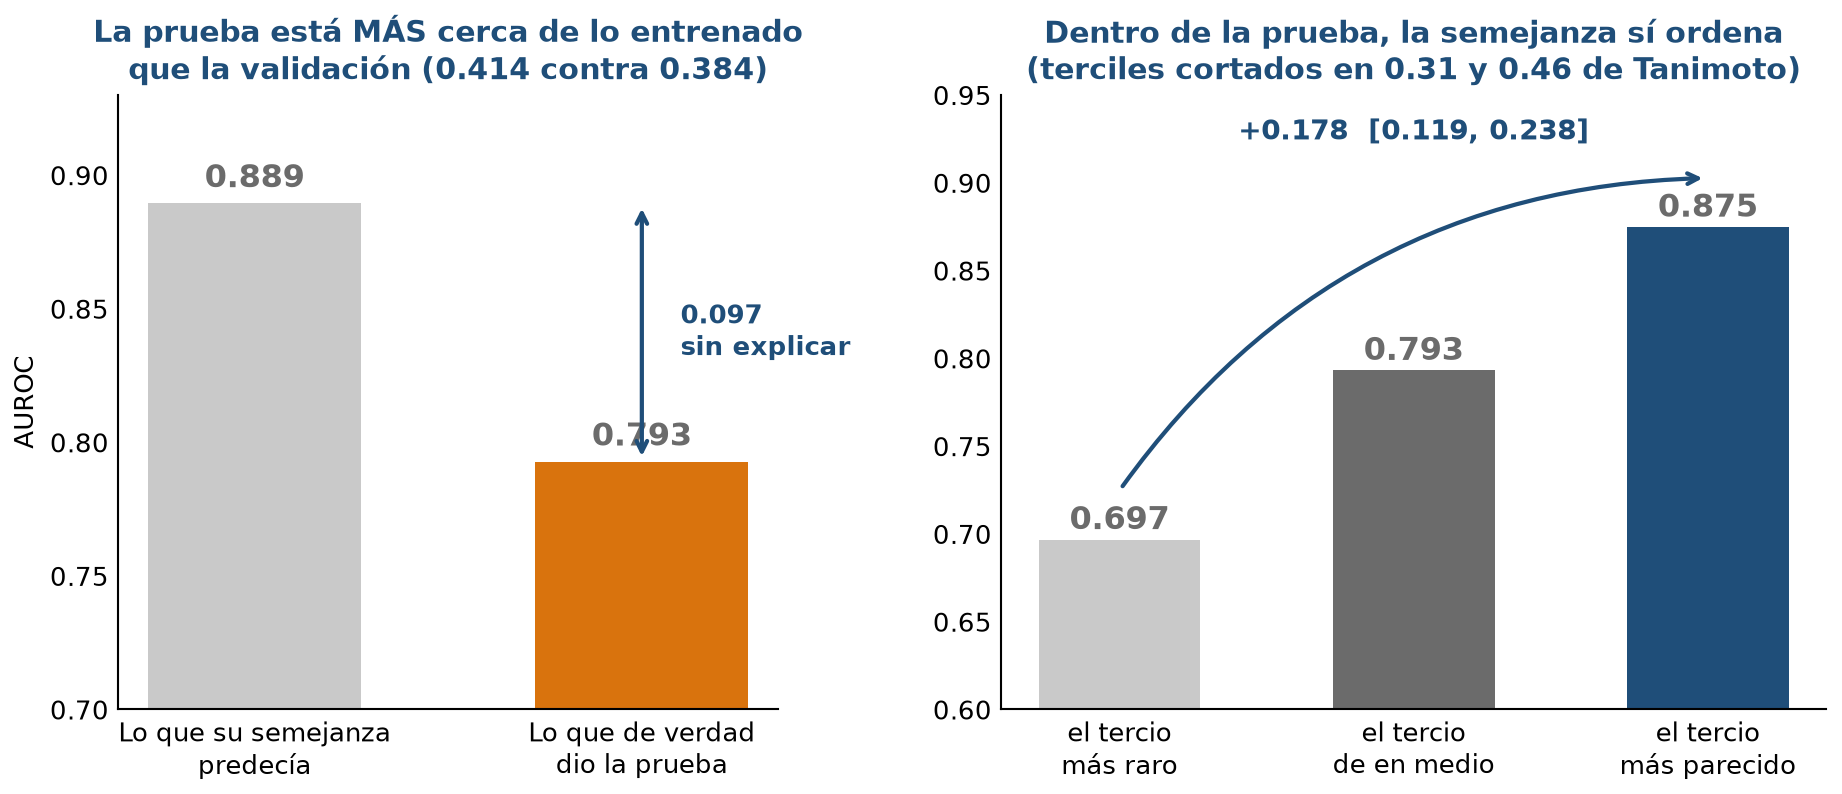
\includegraphics[width=\linewidth,height=9.8cm,keepaspectratio]{dificultad.png}\\[2pt]
  \raggedright\pie{Figura 2. La prueba está más cerca de lo entrenado que la validación, pero rinde 0.097 menos de lo esperado. Dentro de la prueba, la semejanza sí ordena.}
\end{minipage}

\vfill
\begin{minipage}[t]{0.485\linewidth}\centering
  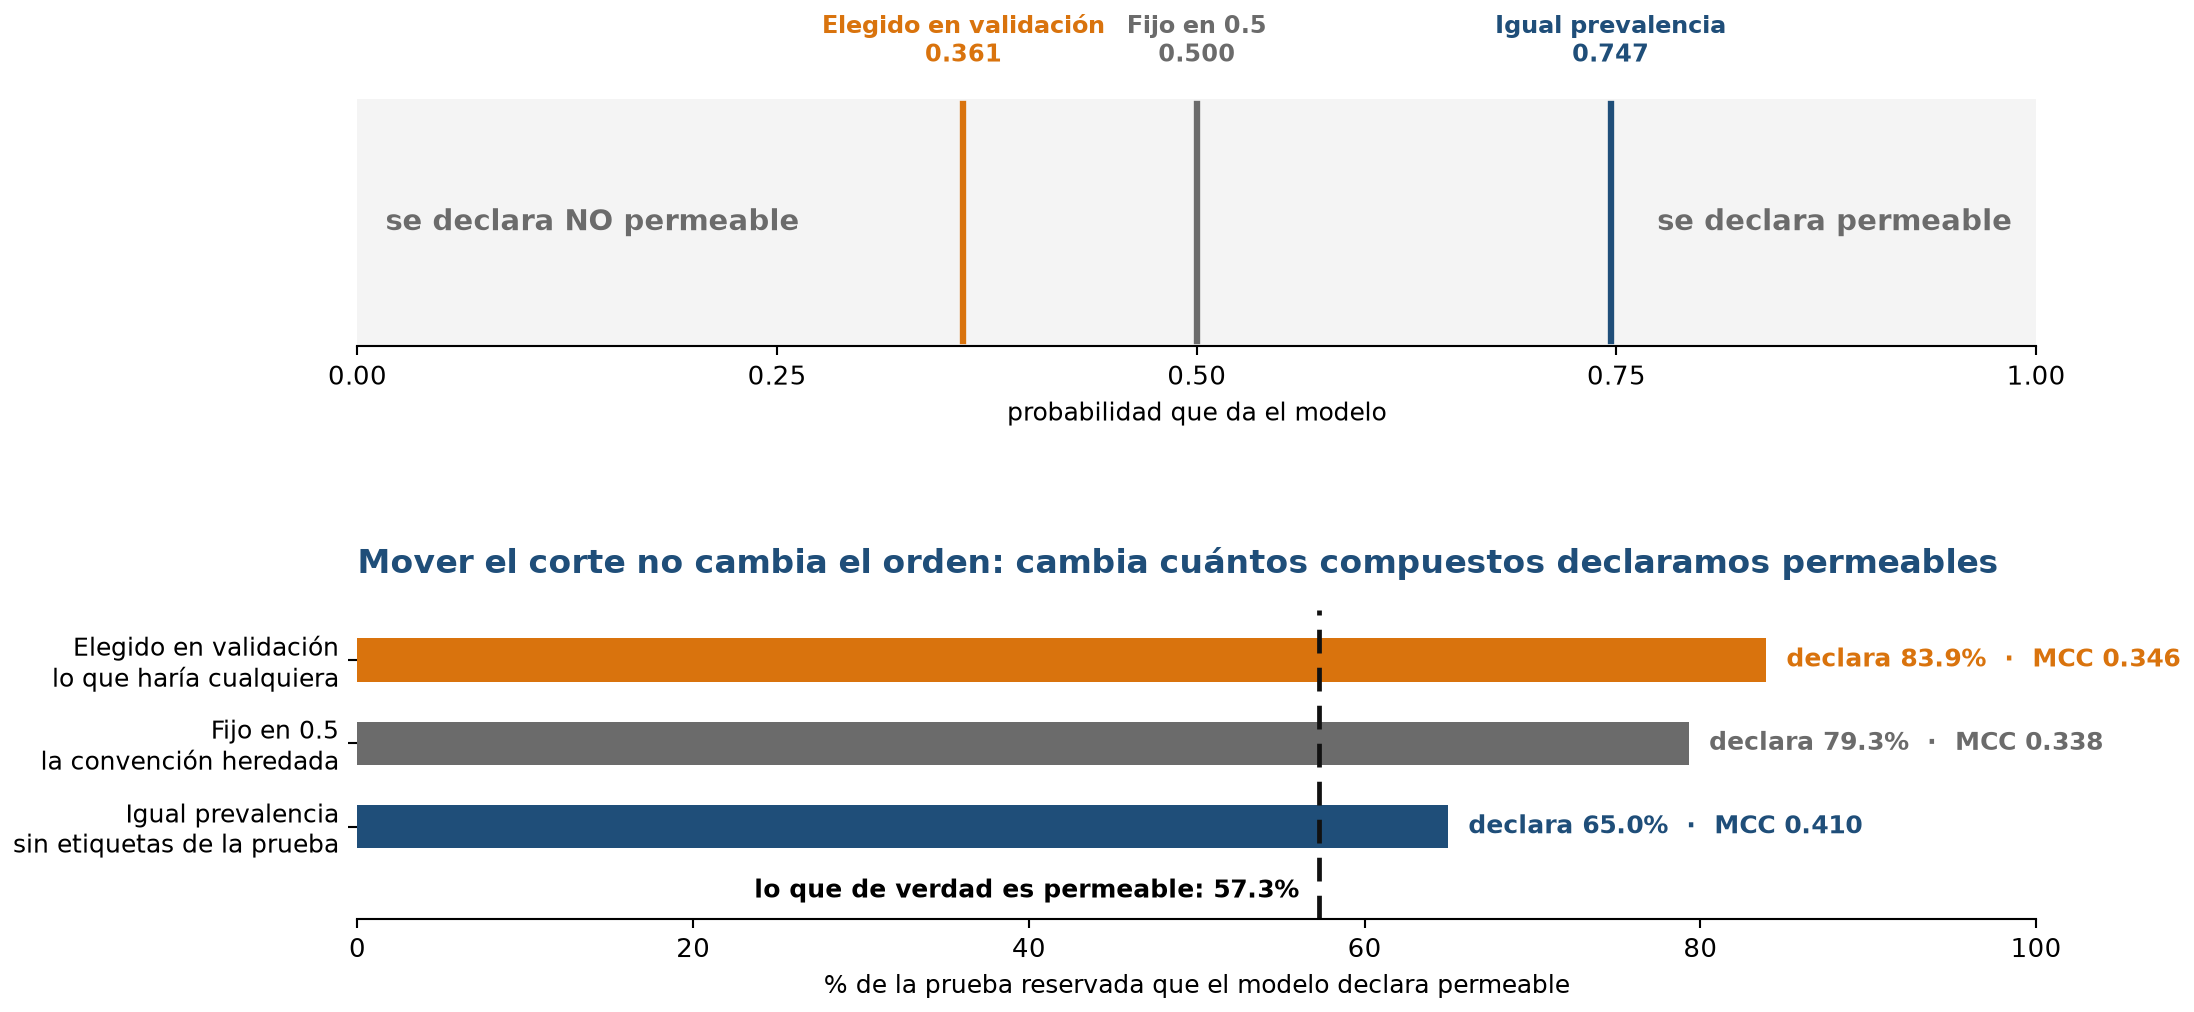
\includegraphics[width=\linewidth,height=9.8cm,keepaspectratio]{corte.png}\\[2pt]
  \raggedright\pie{Figura 3. Mover el corte no cambia el orden: cambia cuántos compuestos se declaran permeables (de 84\,\% a 65\,\%) y el MCC (de 0.346 a 0.410).}
\end{minipage}\hfill
\begin{minipage}[t]{0.485\linewidth}\centering
  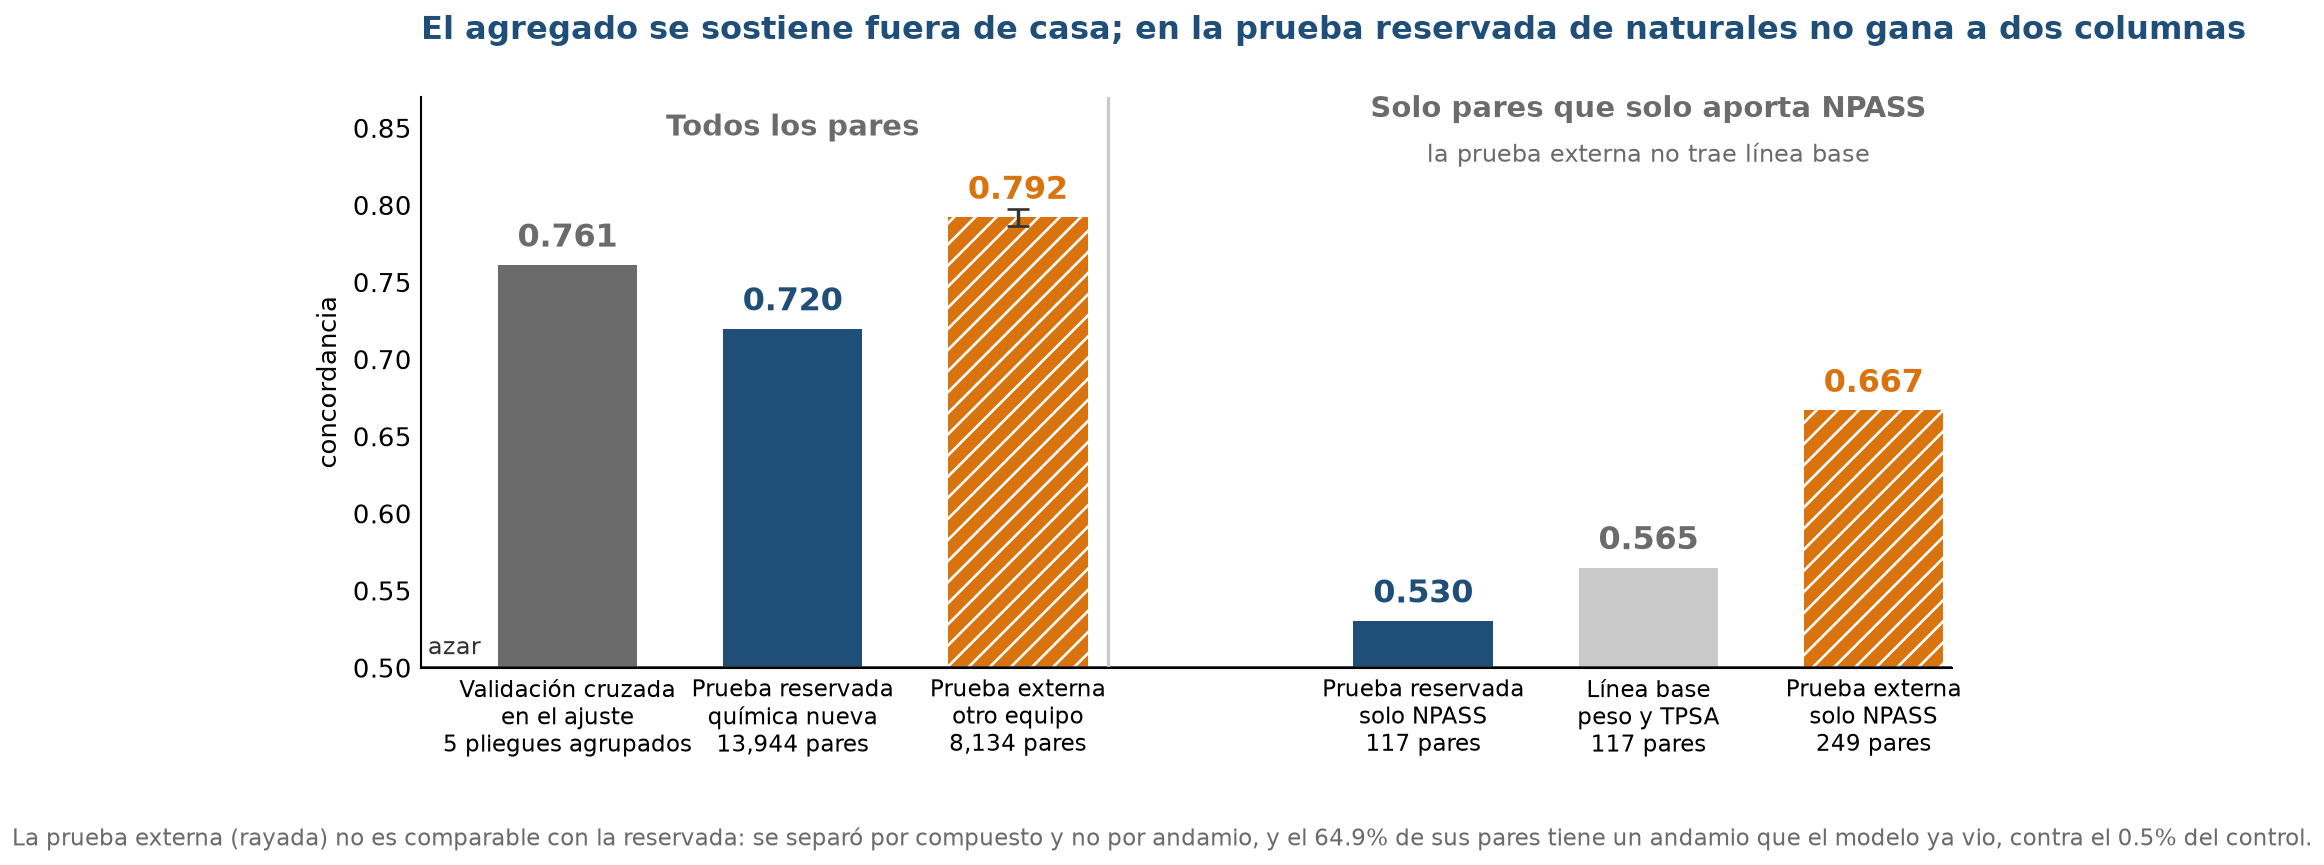
\includegraphics[width=\linewidth,height=9.8cm,keepaspectratio]{fase2_desempeno.png}\\[2pt]
  \raggedright\pie{Figura 4. Fase 2: la concordancia se sostiene en la prueba (0.720). En los 117 pares de naturales, 0.530 (0.511 al reajustar) no se distingue de un modelo de peso y TPSA (0.565).}
\end{minipage}

\vfill
\begin{center}
  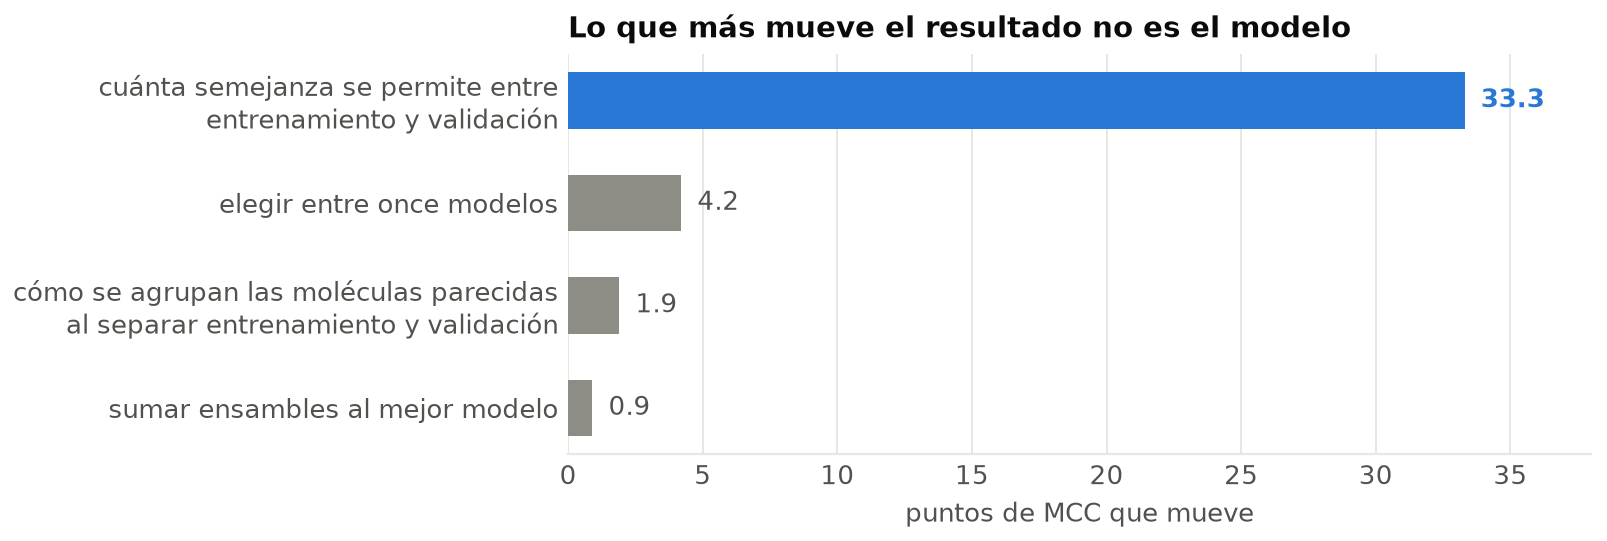
\includegraphics[width=0.84\linewidth,height=8.4cm,keepaspectratio]{f0_palancas.png}\\[2pt]
  \pie{Figura 5. Lo que más mueve el resultado es cuánta novedad se exige, no el modelo.}
\end{center}

\vfill
\end{minipage}\hfill
\begin{minipage}[t][\colh][s]{0.30\linewidth}\cuerpo\vspace{0pt}
% ===== COLUMNA DERECHA =====

\seccion{Conclusiones}
\begin{itemize}[leftmargin=1.2em,itemsep=0.4em]
  \item La confianza en una predicción depende de qué tan nueva es la molécula, no del modelo.
  \item De 0.70 a 0.34 de MCC (acierto en las dos clases) con moléculas nuevas: unos 0.07 eran el corte, que se puede ajustar; el resto sigue sin explicar.
  \item Sirve para ordenar: probar el 70\,\% mejor ordenado conserva el 85.3\,\% de los permeables, 15.3 puntos más que un sorteo.
  \item En naturales el orden de potencia no está demostrado (117 pares). Sigue medirlo con muestras propias y combinar las dos fases.
\end{itemize}

\vfill
\seccion{Qué características pesan}
\begin{center}
  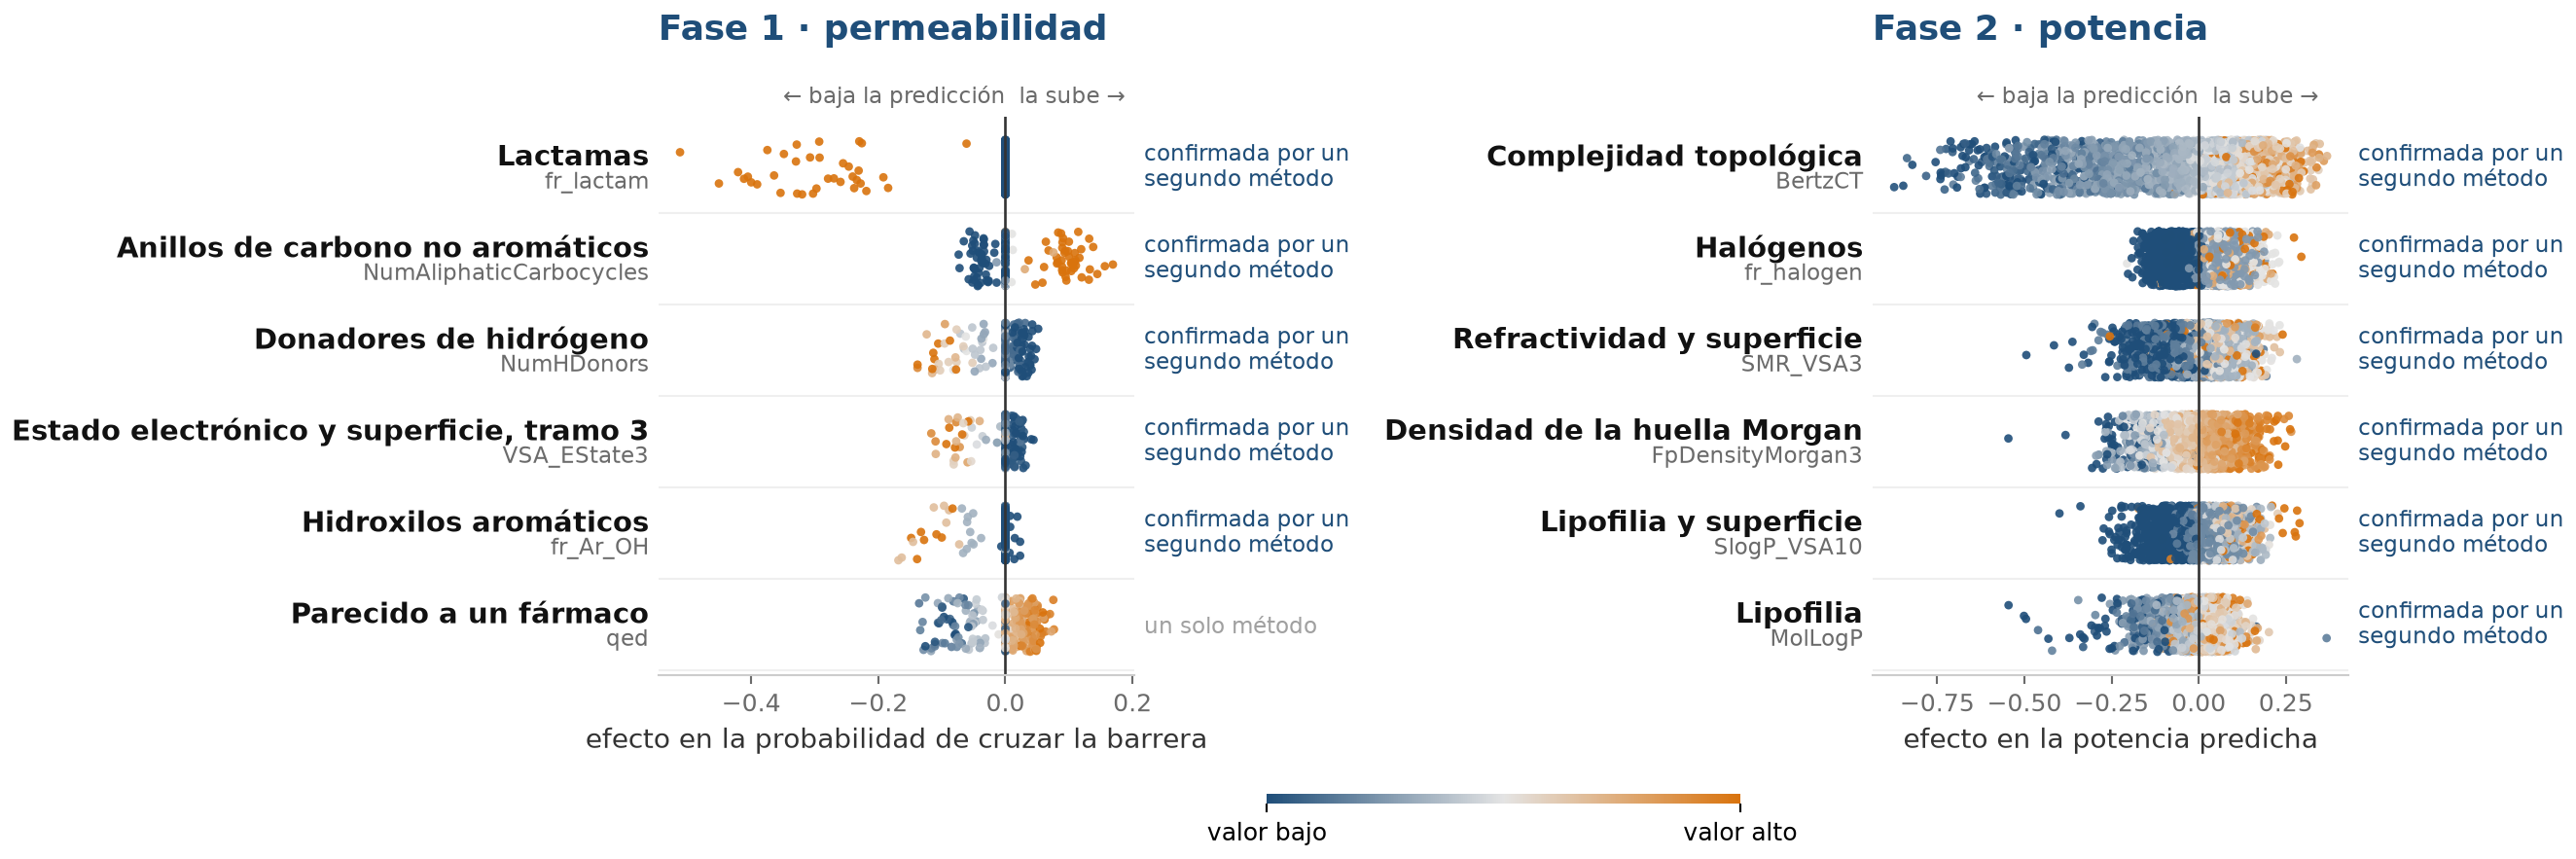
\includegraphics[width=0.9\linewidth,height=7.4cm,keepaspectratio]{importancias_poster.png}\\[2pt]
  \pie{Figura 6. Cada punto es un compuesto o par compuesto-diana. TPSA no domina.}
\end{center}

\vfill
\seccion{Qué entregamos}
\begin{center}
  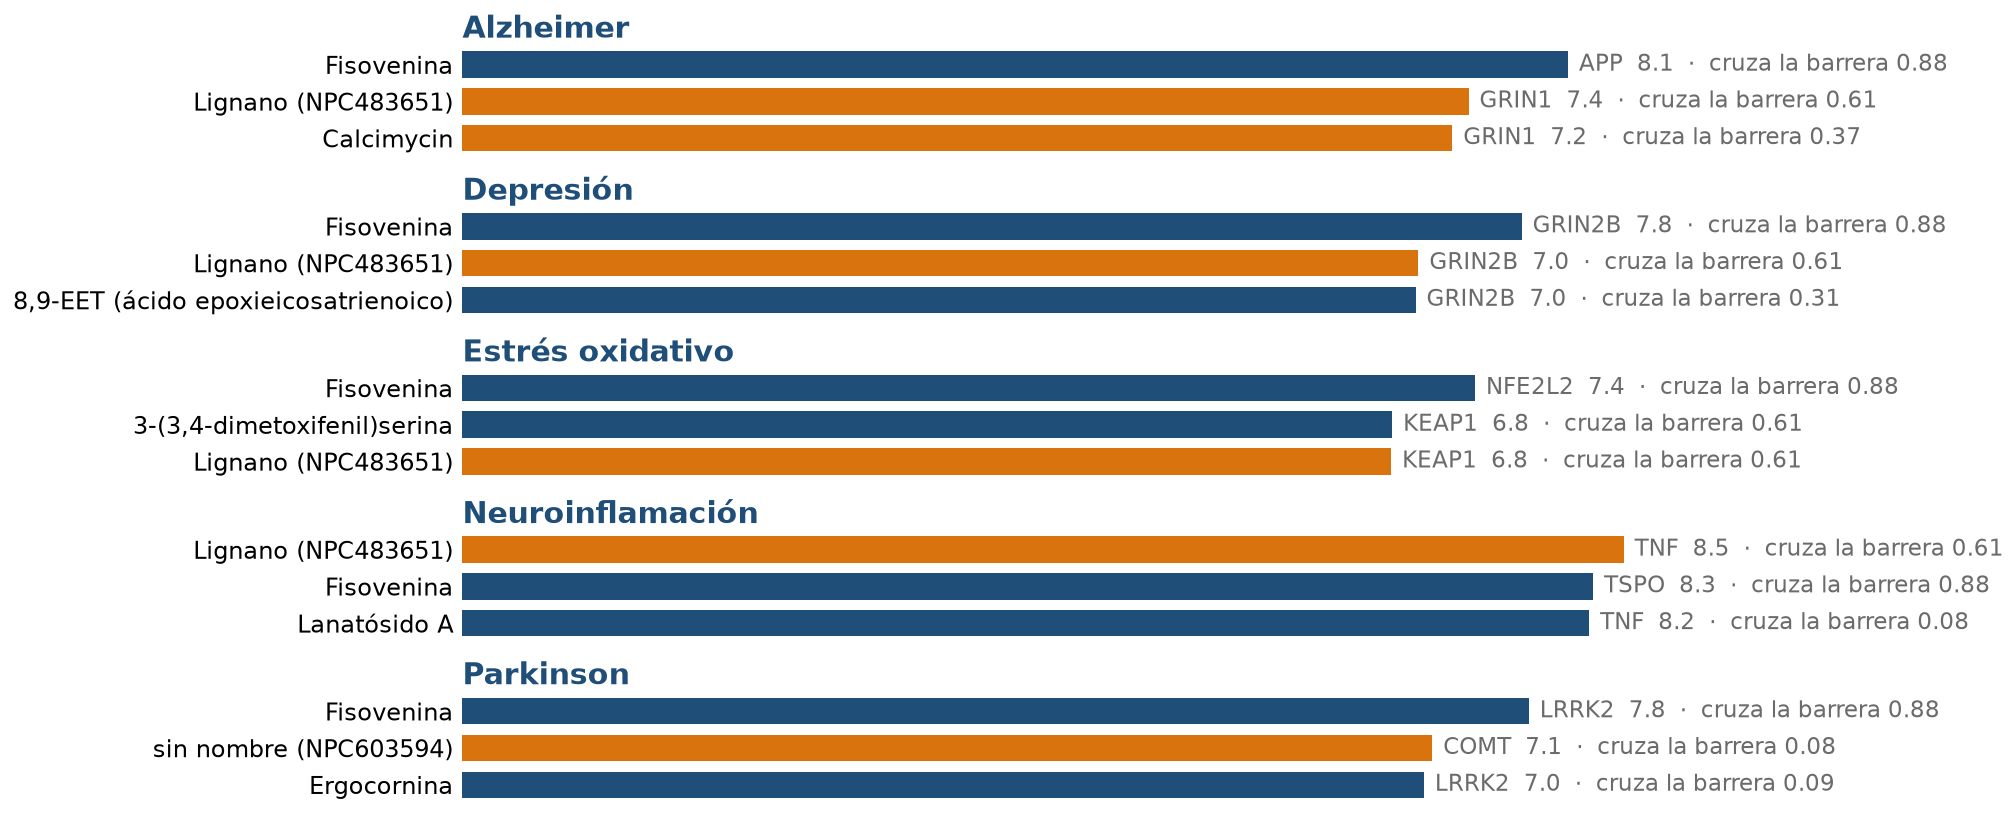
\includegraphics[width=\linewidth,height=5.8cm,keepaspectratio]{lista_priorizada_poster.png}
\end{center}
\begin{itemize}[leftmargin=1.2em,itemsep=0.3em]
  \item Una \href{https://antoniovazquezmartinez.github.io/Bioactive-AI/contenido/lista-priorizada.html}{\underline{lista exploratoria}} de naturales (hipótesis, no resultados) y un \href{https://github.com/AntonioVazquezMartinez/Bioactive-AI/blob/main/notebooks/06_Uso_de_los_modelos.ipynb}{\underline{cuaderno}} para moléculas propias, con aviso si son muy distintas de lo conocido, y una \href{https://github.com/AntonioVazquezMartinez/Bioactive-AI/blob/main/docs/medir-una-representacion.md}{\underline{guía}} para medir columnas nuevas. La continuidad queda con la patrocinadora.
\end{itemize}

\vfill
\seccion{Referencias}
{\fontsize{14}{17}\selectfont
\begin{itemize}[leftmargin=1.2em,itemsep=0.1em]
  \item Meng, F., Xi, Y., Huang, J., y Ayers, P. W. (2021). \emph{A curated diverse molecular database of blood-brain barrier permeability with chemical descriptors.} Scientific Data, 8(1), 289.
  \item Zdrazil, B., et al. (2024). \emph{The ChEMBL Database in 2023.} Nucleic Acids Research, 52(D1), D1180--D1192.
  \item Zhao, H., et al. (2023). \emph{NPASS database update 2023.} Nucleic Acids Research, 51(D1), D621--D628.
\end{itemize}}

\end{minipage}

\vfill
% ---------------------- DECLARACIÓN DE IA ------------------
{\color{olive}\rule{\linewidth}{2.5pt}}
\vspace{0.3cm}

\noindent
{\fontsize{18}{23}\selectfont\color{ink}
{\serif\color{olivedark}\fontsize{22}{28}\selectfont Declaración de uso de inteligencia artificial.}
Anthropic. (2026). \emph{Claude Code} [Agente de programación], con los modelos Claude Opus 5, Claude Sonnet 5.5 y Claude Sonnet 5, https://claude.com/claude-code. Se utilizó para redactar el texto, generar las figuras y calcular las cifras. Las decisiones, la interpretación y las conclusiones son del equipo.
La responsabilidad final sobre el contenido entregado recae en los autores.\par}

\end{document}
